\chapter{Fundamentação Teórica}
\label{cap:fundamentacao}

Nesta seção são detalhados conceitos acerca dos materiais e métodos utilizados na pesquisa. Inicialmente é discorrido sobre o sensoriamento empregado, tipos de sensores, valores aferidos, entre outras características. Posteriormente, é apresentado o modelo matemático \textit{Quarter-Car} (QC), o qual descreve as mecânicas veiculares envolvidas no processo, e sua representação através das variáveis \textit{Golden Car Parameters}. Por fim, são detalhados as técnicas de \textit{Machine Learning} utilizadas com o intuito de reconhecer e classificar os padrões de percepção veicular.

\section{Sensoriamento}

Nesta seção, são apresentados os sensores inerciais, os quais constituem fonte principal de dados do estudo. Em seguida, é discorrido sobre o sensor magnetômetro e GPS, uma vez que servem como sensores auxiliares, comumente utilizados em conjunto com os inerciais para prover informações adicionais. 

\subsection{Sensores Inerciais}

Os sensores inerciais constituem dispositivos que produzem sinais através do princípio da inércia \cite{Braga2017}. Estes sensores compreendem acelerômetros e giroscópios, de um ou mais eixos \cite{Beeby2004}. O acelerômetro mede a força de aceleração (em $m/s^2$ ou g = 9.8 $m/s^2$), enquanto que o giroscópio afere a taxa de rotação (em graus/segundo ou radianos/segundo), ambos sem a necessidade de um referencial externo \cite{Groves2013}. Sendo assim, a partir de um quadro de referência ou posição inicial destes sensores, forças externas que atuam sobre eles causam acelerações e mudanças de orientação (rotação) em um ou mais de seus eixos \cite{Kempe2011}. Em síntese, são sensores que necessitam de movimento para produção de dados. Neste estudo, essas forças são constituídas pela tração do veículo e pelas interações com o ambiente no qual ele trafega.

\subsubsection{Referenciais}

Os sensores inerciais não requerem nenhum referencial externo. Sendo assim, possuem seu próprio referencial, onde o sistema de coordenadas no qual os dados são amostrados é definido em relação a si próprios. No entanto, a análise dos dados com o objetivo de produzir percepção veicular deve ser realizada no referencial do veículo, como mostra a Figura \ref{fig:quadros_referencia}. Para isso, é necessário reorientar os eixos, mapeando os dados brutos de um sistema para outro.

\begin{figure}[h!]
  \centering
  \caption{Referenciais: (a) Referencial do sensor. (b) Referencial do sensor interno a dispositivos móveis. (c) Referencial da Terra. (d) Referencial do veículo.}
   \label{fig:quadros_referencia}
   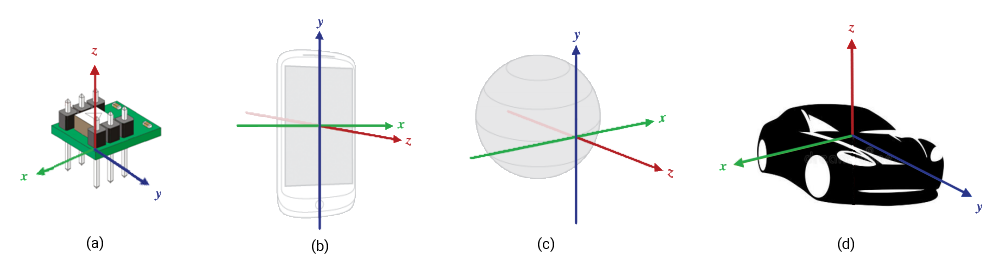
\includegraphics[width=1\textwidth]{figuras/fig2.png}
   \fonte{O autor.}
\end{figure}

A orientação dos dados é importante no processo de análise para que se possa utilizar os valores de acordo com o tipo de percepção a ser realizada. Sendo assim, baseando-se no referencial do veículo, os padrões de percepção de ambiente são mais evidentes na aceleração do eixo Z e na taxa de rotação do eixo Y. Já quanto aos padrões de propriocepção, mostram-se mais evidentes nos dados de aceleração nos eixos X e Y e nas taxas de rotação dos eixos X e Z. Para uma padronização de nomenclatura neste trabalho, serão usados os termos definidos nas Tabelas \ref{table:accelerometer_reference_frames} e \ref{table:gyroscope_reference_frames} para se referir aos dados em relação a cada um dos referenciais.

\begin{table}[h!]
    \caption{Referenciais para os dados de aceleração.}
    \label{table:accelerometer_reference_frames}
    \centering
    \small
    \begin{tabular}{clll}
        \toprule
        \textbf{Axis} & \textbf{Sensor} & \textbf{Veículo} & \textbf{Mundo} \\
        \toprule
        X & Aceleração em X & Aceleração Lateral & Aceleração Leste \\
        \midrule
        Y & Aceleração em Y & Aceleração Longitudinal & Aceleração Norte \\
        \midrule
        Z & Aceleração em Z & Aceleração Vertical & Aceleração Vertical (Mundo) \\
        \bottomrule
    \end{tabular}
    \fonte{O autor.}
\end{table}

\begin{table}[h!]
    \caption{Referenciais para os dados de taxa de rotação.}
    \label{table:gyroscope_reference_frames}
    \centering
    \small
    \begin{tabular}{clll}
        \toprule
        \textbf{Axis} & \textbf{Sensor} & \textbf{Veículo} & \textbf{Mundo} \\
        \toprule
        X & Taxa de Rotação Pitch & Taxa de Rotação Lateral & N/A \\
        \midrule
        Y & Taxa de Rotação Roll & Taxa de Rotação Longitudinal & N/A \\
        \midrule
        Z & Taxa de Rotação Yaw & Taxa de Rotação Vertical & N/A \\
        \bottomrule
    \end{tabular}
    \fonte{O autor.}
\end{table}

Para a reorientação dos eixos, duas estratégias foram identificadas nos estudos revisados: o posicionamento controlado e o mapeamento através de fórmulas baseadas nos ângulos de Euler. O posicionamento controlado consiste em uma técnica simples, onde sensor é colocado no veículo de forma que os eixos nos referenciais coincidam, ou seja, os eixos do sensor ficam alinhados com os eixos do veículo. Portanto, não é necessário aplicar pré-processamento para reorientação. Essa técnica é usada tanto para os dados do acelerômetro e do giroscópio. 

Os ângulos de Euler, por sua vez, aplicados apenas aos dados de aceleração, fornecem um meio de representar a orientação espacial tridimensional de qualquer referencial como uma composição de três rotações elementares. A orientação de referência pode ser tomada como uma orientação inicial a partir da qual o sistema de coordenadas gira para alcançar sua orientação real \cite{Singh2017}. Assim, essas fórmulas reorientam os dados brutos usando os ângulos fornecidos. Estes dois métodos são detalhados e analisados comparados no Capítulo \ref{cap:revisao}, em conjunto com as demais análises da literatura. 

\subsubsection{Fatores de Dependência}

Os valores amostrados através dos sensores inerciais, embora não dependam de um referencial externo para sua produção, são afetados por propriedades externas e internas aos sensores. Essas propriedades constituem fatores de dependência, que influenciam diretamente a amplitude e dispersão dos valores medidos. Através da tanto da análise da literatura, quando de experimentos exploratórios conduzidos, foi possível observar a existência de fatores de dependência classificados na forma de quatro propriedades, discutidas a abaixo. Para que uma solução desenvolvida possa ser adaptativa na forma que está sendo proposta, é necessário que o modelo considere todas estas propriedades no seu desenvolvimento.

\begin{description}
	
	\item [Propriedades Sensoriais:] 
	
	Quatro fatores de dependência estão relacionados às configurações e características dos sensores, sendo eles a orientação \cite{Kumar2017}, resolução, faixa de medição e taxa de amostragem. A orientação do sensor, conforme discutido na seção anterior, afeta a amostragem de dados no sistema de coordenadas correto. Portanto, o sensor deve ser colocado de forma a ficar alinhado com o sistema de coordenadas do veículo ou ter uma reorientação de eixos para esse referencial. Isso implica na confiabilidade dos dados existentes em cada eixo de análise, pois cada um deles visa atingir certa percepção veicular.

	O segundo e o terceiro fator estão fortemente correlacionados. A resolução é definida de acordo com a faixa de medição escolhida para o sensor. Portanto, é necessário que o sensor tenha uma faixa de medição adequada para poder amostrar os dados sem saturar, ou seja, que a faixa de medição do sensor não seja menor que os valores possíveis a serem monitorados. A resolução, estabelecida a partir da faixa de valores a serem analisados, fornece o quão próximo o valor medido é comparado ao valor real, no processo de quantização. Assim, devido à limitação do número de bits representado pelos sensores, quanto maior a faixa de medição, menor a resolução.
	
	Por fim, a taxa de amostragem descreve a frequência da amostragem de dados por segundo. A escolha desse valor deve levar em consideração não apenas o custo computacional de armazenamento e processamento dos dados amostrados, mas também se, a uma determinada velocidade, será possível obter amostras suficientes para realizar as percepções. Dessa forma, quando o veículo está em alta velocidade, percepções transientes, como buracos, precisam de uma taxa de amostragem satisfatória, para que seja possível adquirir alguma amostra desse evento.
	
	\item [Propriedades Veiculares:] em relação às mecânicas veiculares, o principal fator de dependência é o sistema de suspensão veicular \cite{Kumar2017, Wickramarathne2018}. O sistema de suspensão do veículo, com o objetivo de amortecer os impactos causados pela superfície da pista, faz com que os valores absolutos sejam reduzidos quando medidos acima da suspensão, como ocorre quando os sensores são embarcados em dispositivos móveis. Portanto, os valores amostrados nos sensores anexados no veículo abaixo da suspensão não apresentam essa interferência, embora ainda recebam um pequeno amortecimento causado pelo pneu. Sendo assim, para realizar as percepções em diferentes veículos, deve-se considerar que cada um possui um sistema de suspensão diferente, sendo mais ou menos eficiente.

	\item [Propriedades Ambientais:] estas propriedades não abordadas em trabalhos relacionados, não são tão evidentes, embora necessitem ser consideradas na modelagem da adaptação. Seus fatores de dependência se relacionam com questões climáticas, como superfície de pista com água ou de pouco atrito, que levam a aquaplanagem e derrapagem. Sendo assim, são percepções que implicam na percepção de outras, ou seja, percepções que dependem de percepções. O mesmo ocorre com a variabilidade de superfície, onde a identificação de eventos transientes como buracos e lombadas dependem diretamente do tipo de pavimento que existe na pista, e se existe. Da mesma forma, o dinamismo do estado de conservação de um tipo de pavimento deve ser considerado para detectá-lo corretamente.

	\item [Propriedades de Condução:] as propriedades de condução, intrinsecamente relacionadas as propriedades veiculares, dizem respeito as ações de quem controla o veículo. Nesse sentido, o principal fator de dependência a ser considerado é a velocidade longitudinal \cite{Brunauer2016, Douangphachanh2013, Gueta2017, Kumar2017, Lima2016, M.2017, Nalavde2015, Singh2017}. A velocidade do veículo possui duas implicações. Uma vez que as curvas são feitas em todos os eixos do sistema de coordenadas do veículo, ocorre a produção do componente de força centrífuga. Portanto, as acelerações medidas dependem diretamente da velocidade aplicada. A segunda implicação da velocidade está na distribuição no tempo dos valores amostrados. Em velocidades mais baixas, mais amostras do evento são coletadas e, com o veículo em velocidades diferentes, diferentes quantidades de amostras são obtidas.

\end{description}

% \subsection{Magnetômetro}

% O magnetômetro é um sensor auxiliar comumente embarcado com os sensores inerciais devido sua função. Este sensor mede o campo geomagnético ambiental (em $\mu$T) em seus três eixos físicos \cite{Sattar2018}. Sendo assim, é geralmente aplicado junto aos ângulos de Euler para dar orientação aos dados e empregado com os dados de aceleração para aproximar dados de localização e velocidade mais rapidamente, uma vez que a taxa de amostragem do GPS é pequena.

\subsection{GPS}

O Sistema de Posicionamento Global (\textit{Global Positioning System} - GPS) consiste de um sistema de satélites que orbitam o planeta, auxiliando receptores em terra a determinar sua localização \cite{Milette2012}. Sendo assim, além dos dados geodésicos de latitude e longitude, o receptor GPS também afere sua velocidade. Embora preciso, este sistema possui uma taxa de amostragem baixa em relação aos demais sensores, cerca de 1Hz.

\section{Quarter Car}

O modelo matemático \textit{Quarter Car} (QC) descreve as variáveis da dinâmica veicular, conforme ilustra a Figura \ref{fig:quarter_car}. O modelo QC possui propriedades relacionadas a roda, suspensão e amortecimento. A propriedade de massa suspensa do veículo (Ms), fica acima da suspensão e representa um quarto da massa veicular. A propriedade de massa não suspensa (Mu), abaixo da suspensão, inclui a massa de uma roda e do sistema de suspensão conectado a ela. Entre as massas, existe a suspensão feita da mola (Ks) e de um amortecedor (C), que suporta a massa suspensa. Uma vez que a massa não suspensa está em contato direto com a superfície da pista, existe a rigidez do pneu (Kt) e a capacidade de absorção do pneu (Ct) impactando nos valores de força \cite{Yafeai2019}.

\begin{figure}[h!]
  \centering
  \caption{O modelo Quarter Car.}
   \label{fig:quarter_car}
   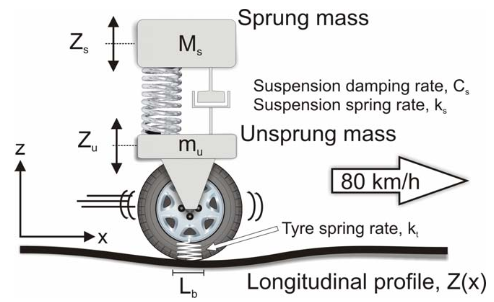
\includegraphics[width=0.6\textwidth]{figuras/fig2_2.png}
   \fonte{\cite{Loizos2008}}
\end{figure}

Através das diversas fórmulas que compõem o modelo, foram criados valores padrões para estas propriedades, denominados \textit{Golden Car Parameters} \cite{Loizos2008}, conforme detalha a Tabela \ref{table:golden_car_parameters}.

\begin{table}[h!]
    \caption{Os parâmetros Golden Car.}
    \label{table:golden_car_parameters}
    \centering
    \small
    \begin{tabular}{clll}
        \toprule
        \textbf{Parâmetro} & \textbf{Valor} \\
        \toprule
        Ks/Ms & 63,3 \\
        \midrule
        Kt/Ms & 653 \\
        \midrule
        Cs/Ms & 6 \\
        \midrule
        Mu/Ms & 0,15 \\
        \bottomrule
    \end{tabular}
    \fonte{\cite{Loizos2008}}
\end{table}

\section{Técnicas Clássicas de Machine Learning}

Com o desenvolvimento da Inteligência Artificial, diversas técnicas surgiram para classificação, regressão e previsão. Dentre as técnicas clássicas de clustering e aprendizado de máquina supervisionado, neste trabalho foram utilizadas as técnicas K-Means Clustering (KMC), K-Nearest Neighbors (KNN) e Support Vector Machines (SVM), detalhadas nas próximas subseções.

\subsection{K-Means Clustering}

O KMC consiste de uma técnica não supervisionada para clustering, que permite identificar agrupamentos de dados semelhantes. Neste método, cada dado é atribuído a um dos k clusters baseando-se em uma métrica de distância, como a Euclidiana, em relação à centroide do cluster. Iterativamente, a centroide de cada clusters é recalculada com base na média dos dados, e as distâncias novamente recalculadas, até que as centróides sejam estabilizadas, ou o número máximo de iterações atingido \cite{foley2019,nisbet2009}.

\subsection{K-Nearest Neighbors}

O KNN consiste de uma técnica para classificação a qual se baseia em métricas de similaridades entre os dados para reconhecer padrões. Desta forma, para um novo dado é calculada a distância entre ele e cada um dos dados de treinamento, identificando os k vizinhos mais próximos. A classe do novo dado é definida como aquela mais comum entre seus k vizinhos \cite{Khandelwal2018}.

\subsection{Support Vector Machines}

O SVM é uma técnica de aprendizado supervisionado aplicados em classificação, onde o algoritmo busca por um optimal hyperplane que separa as classes de dados. Em problemas não lineares, como é o caso deste, é necessário a utilização do hiperparâmetro kernel, o qual converte problema não separável em problema separável, para que o SVM possa classificar \cite{Shubham2018}.

\section{Técnicas de Deep Learning}

Com o desenvolvimento do aprendizado de máquina, especialmente a partir de 2006, surgiu nesta área um segmento denominado aprendizado profundo (\textit{Deep Learning}) \cite{Deng2014}. Até então, a extração características importantes que bem representassem os dados parametrizados à uma técnica de reconhecimento de padrões, constituía um problema central. Sendo assim, as técnicas existentes apresentavam a grande dificuldade de se extrair, em um pré-processamento, características de alto nível através de dados brutos \cite{Goodfellow2016}. 

Com o desenvolvimento do \textit{Deep Learning}, esse problema foi solucionado, sendo introduzidas representações que são expressadas em termos de outras, construindo conceitos complexos através de conceitos simples \cite{Goodfellow2016}. Nessa abordagem, tornou-se possível construir modelos computacionais compostos de múltiplas camadas de processamento para aprender a representação dos dados com diversos níveis de abstração \cite{LeCun2015}. Sendo assim, o aprendizado profundo descobre uma estrutura complexa em grandes conjuntos de dados usando o algoritmo de retropropagação para calcular como alterar seus parâmetros internos, os quais são usados para calcular a representação em cada camada a partir da representação na camada anterior \cite{LeCun2015}.

Com este novo paradigma, foram melhorados drasticamente o estado da arte em reconhecimento de fala, reconhecimento visual de objetos, detecção de objetos e muitos outros domínios \cite{LeCun2015}. Os diversos métodos presentes nessa categoria podem ser classificados entre redes profundas para aprendizado não supervisionado ou generativo, redes profundas para aprendizado supervisionado e redes profundas híbridas \cite{Deng2014}. Neste trabalho, foram utilizadas redes  profundas para aprendizado supervisionado do tipo \textit{Long Short-Term Memory} (LSTM) e \textit{Convolutional Neural Network} (CNN), assim como redes profundas híbridas CNN-LSTM, discorridas nas próximas seções.

\subsection{Long Short-Term Memory}

A \textit{Long Short-Term Memory} (LSTM) constitui um tipo de Rede Neural Recorrente (\textit{Recurrent Neural Network} - RNN) considerada ideal para predição e classificação de séries temporais, substituindo muitas abordagens tradicionais por \textit{Deep Learning} \cite{Zaccone2017}. Nesta abordagem, introduzindo o conceito de célula de memória e auto-loops conforme a Figura \ref{fig:cell_lstm}, a rede pode manter valores por um período curto ou longo, como uma função de suas entradas. Assim, a célula consegue se lembrar daquilo que é importante, e não apenas do último valor computado \cite{Jones2017}.

\begin{figure}[h!]
  \centering
  \caption{Célula de memória da LSTM com auto-loop.}
   \label{fig:cell_lstm}
   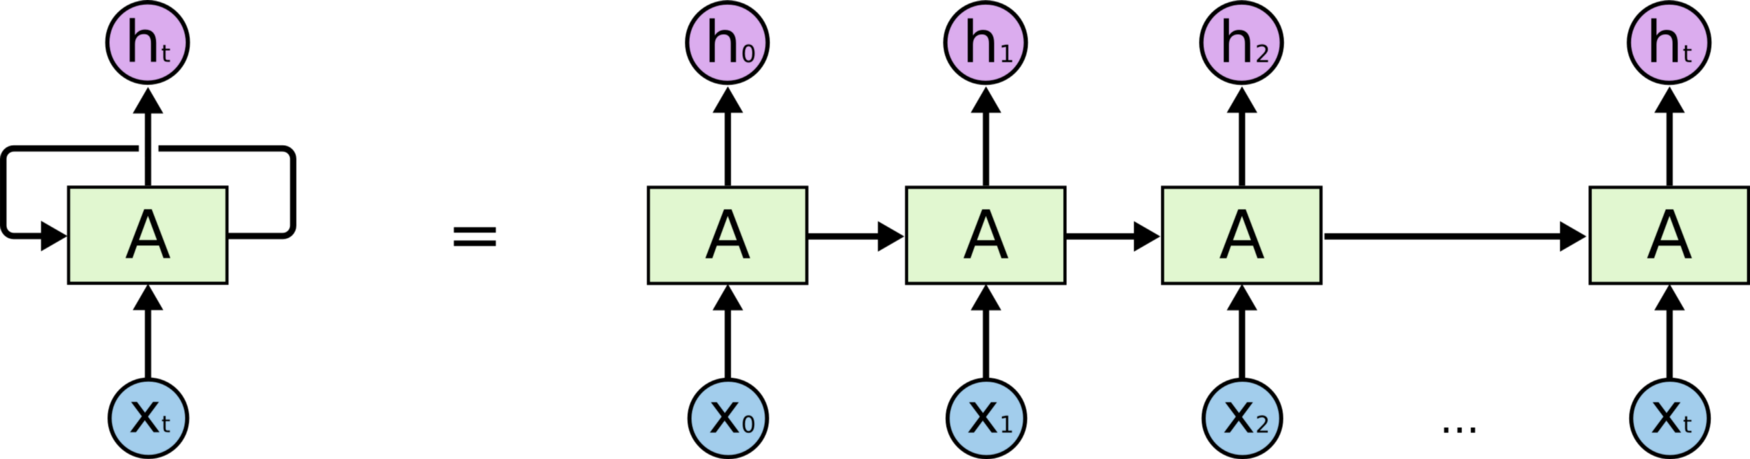
\includegraphics[width=1\textwidth]{figuras/fig2_3.png}
   \fonte{\cite{Junior2019}}
\end{figure}

Cada célula de memória de uma LSTM possuí três portas que controlam o fluxo de informações para dentro e fora da célula. Estas são a porta de entrada (\textit{input gate}), a porta de saída (\textit{output gate}) e a porta de esquecimento (\textit{forget gate}). As portas possuem pesos, onde os valores computados seguem um fluxo no qual resultam em alterações no estado de célula. Sendo assim, inicialmente tem-se a porta de esquecimento, responsável por decidir quais dados devem ser mantidos na memória e quais devem ser esquecidos \cite{Nguyen2018}. Isso permite que a célula se lembre de dados anteriores importantes, ou apenas de novos dados, esquecendo os anteriores. Em seguida, a porta de entrada é responsável por controlar quando novas informações podem entrar na memória. Finalmente, a porta de saída controla quais as informações contidas no próximo estado da célula.\cite{Jones2017}

\begin{figure}[h!]
  \centering
  \caption{Portas da célula de memória da LSTM.}
   \label{fig:cell_lstm_gates}
   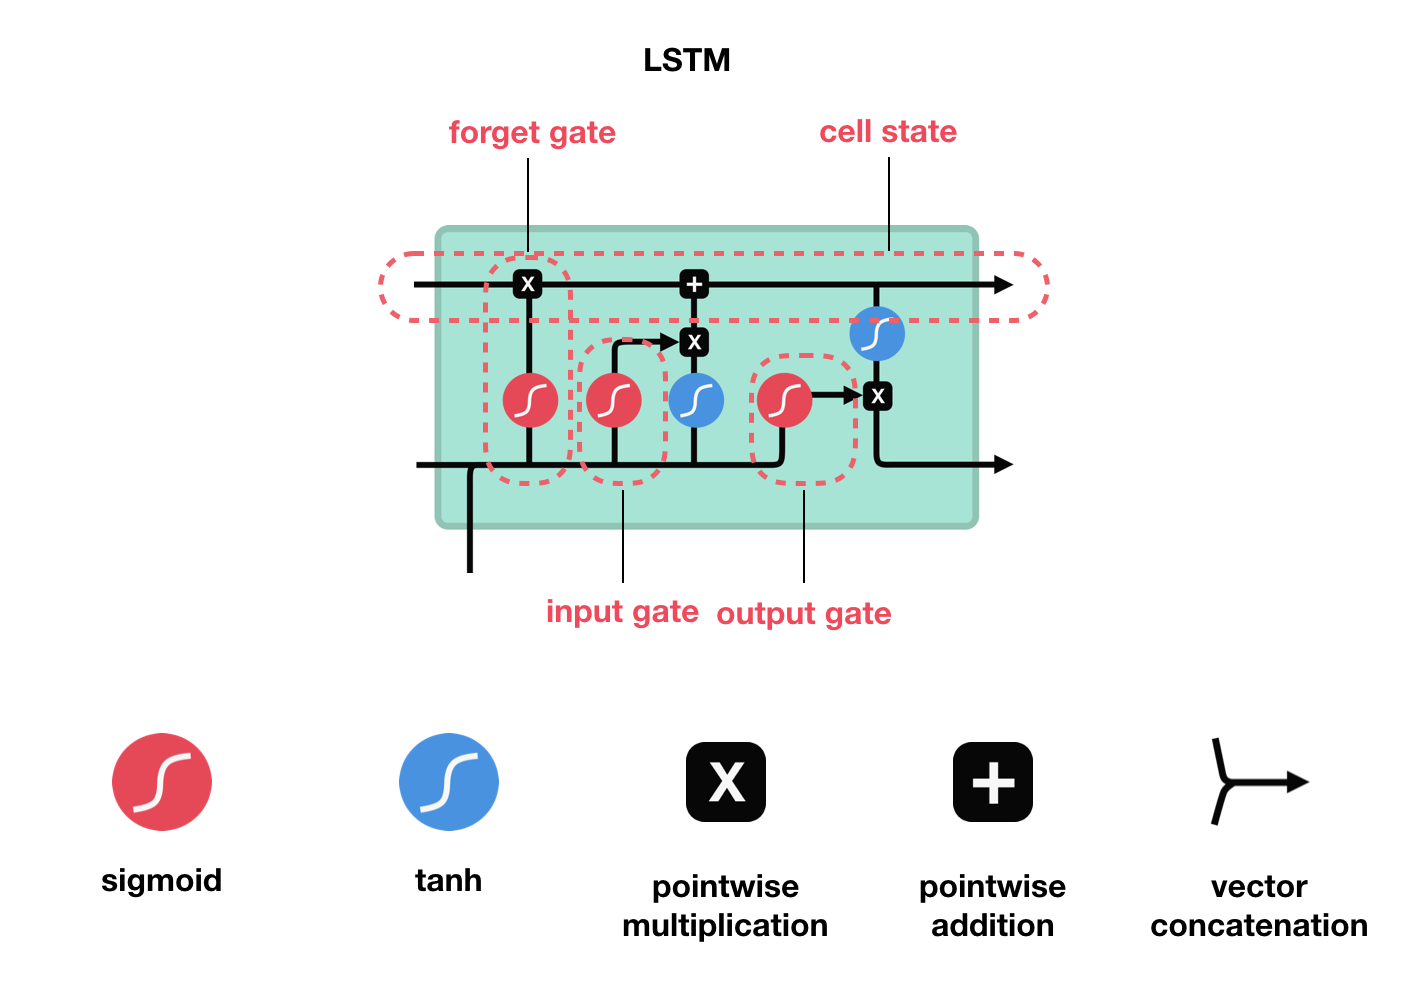
\includegraphics[width=1\textwidth]{figuras/fig2_3_1.png}
   \fonte{\cite{Nguyen2018}}
\end{figure}

\subsection{Convolutional Neural Network}

A CNN é um tipo de rede neural capaz de extrair características diretamente dos sinais, através de convoluções \cite{Dixon2019}. Quando aplicada à classificação de séries temporais, a CNN tem duas vantagens em relação a outras técnicas: dependência local, uma vez que os sinais próximos provavelmente estão correlacionados; e invariância de escala para diferentes passos ou frequências \cite{Wang2019}. Neste tipo de rede, cada camada de convolução possuí uma quantidade n de filtros aplicados com um kernel de tamanho m, conforme ilustra a \autoref{fig:cnn_convolution} e \autoref{fig:cnn_convolution_3d}. Após a convolução, geralmente existem camadas de pooling e fully connected, que executam tarefas de classificação \cite{Wang2019}.

\begin{figure}[h!]
  \centering
  \caption{Convolução em dados 1D.}
   \label{fig:cnn_convolution}
   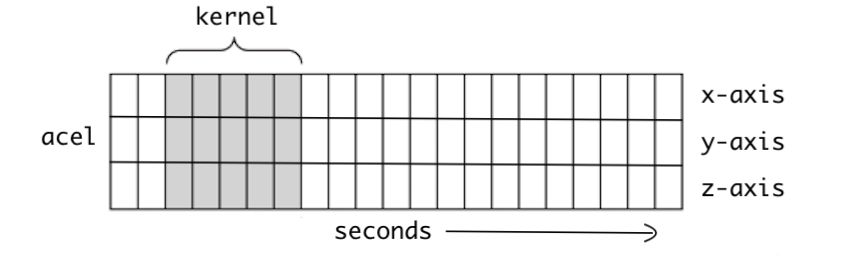
\includegraphics[width=0.9\textwidth]{figuras/cnn_kernel.png}
   \fonte{\cite{Verma2020}}
\end{figure}

\begin{figure}[h!]
  \centering
  \caption{Convolução em dados 3D.}
   \label{fig:cnn_convolution_3d}
   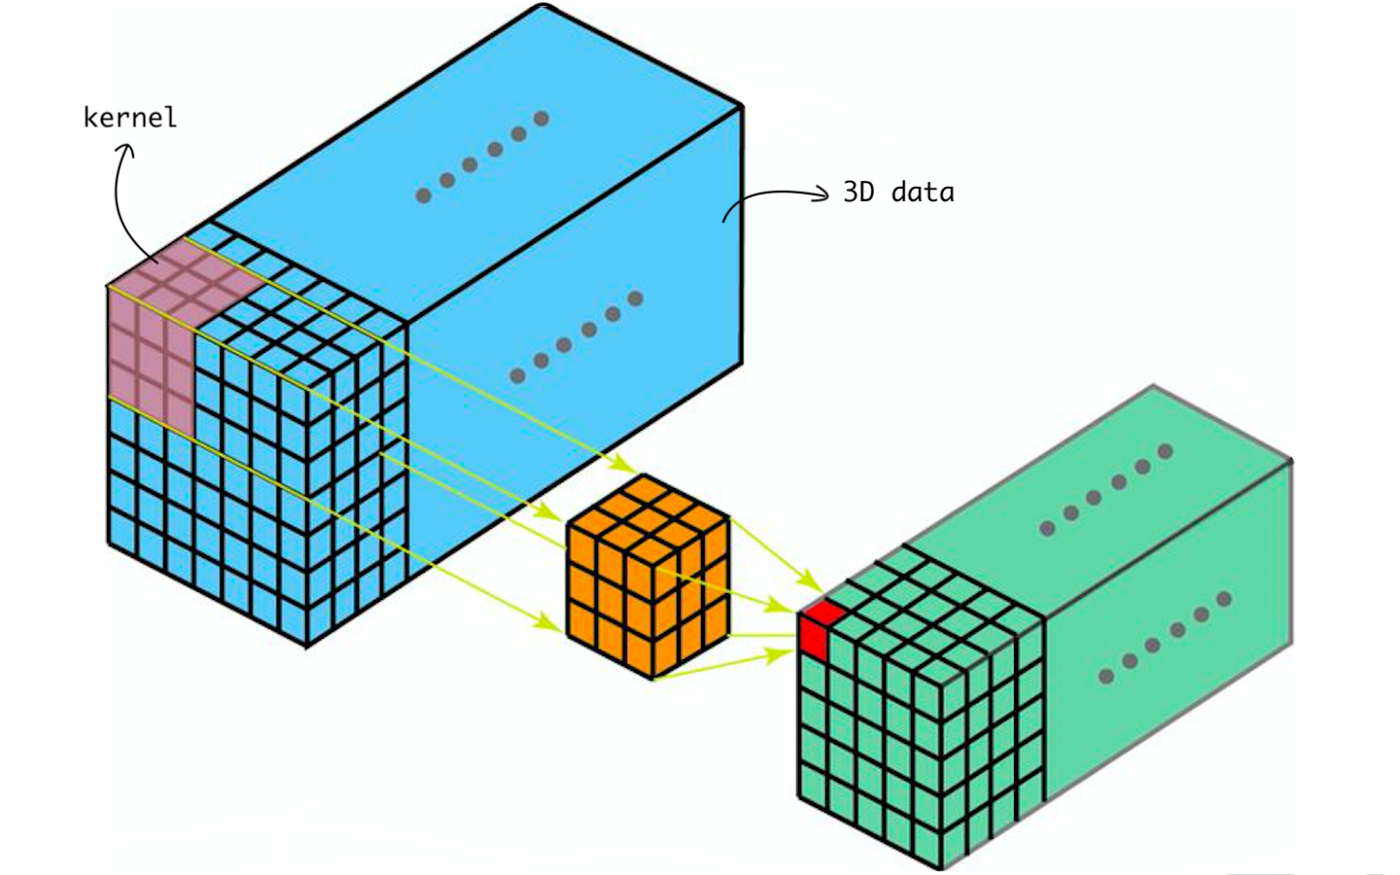
\includegraphics[width=0.8\textwidth]{figuras/cnn_3d.png}
   \fonte{\cite{Verma2020}}
\end{figure}

\subsection{CNN-LSTM}

As redes do tipo CNN-LSTM-based constituem modelos híbridos que utilizam de ambas camadas de convolução e recorrência \cite{Deep2019}. Nestas redes, os sinais são inicialmente agrupados em janelas de dados, e cada janela em blocos menores. Sendo assim, cada bloco é processado por camadas de convolução que fazem a extração de características complexas \cite{Deep2019}. Em seguida, esses blocos são entregues as camadas de recorrência, para interpretar a sequência temporal das características.